\documentclass{article}
\usepackage{tikz,amsmath,amsthm,tkz-graph,algpseudocode}
\usetikzlibrary{positioning}
\tikzset{box/.style={draw, thick, text centered, minimum height=0.5cm, minimum width=1cm}}
\tikzset{line/.style={draw, thick, -latex'}}
\title{CSC 226 Problem Set 3 Written Part}
\renewcommand{\thesubsection}{\thesection.\alph{subsection}}
\author{%
	Oliver Tonnesen\\
	V00885732}
\date{November 8, 2018}
\begin{document}
\maketitle
\section{Listing vertices of a negative cycle}
The following is a slight variation of the Bellman-Ford algorithm.
\begin{algorithmic}[1]
	\Function{FindNegCycle}{G}
	\State $d\gets$int array
	\State $\pi\gets$vertex array
	\For{$v$ in $V$}
		\State $d[v]\gets\infty$
		\State $\pi[v]\gets$null
	\EndFor
	\State $d[0]\gets0$
	\For{$i\gets0,1,\ldots,|V|-2$}
		\For{$e$ in $E$}
			\If{$d[e.u]+e.w<d[e.v]$}
				\State $d[e.v]\gets d[e.u]+e.w$
				\State $\pi[e.v]\gets e.u$
			\EndIf
		\EndFor
	\EndFor
	\For{$e$ in $E$}
		\If{$d[e.u]+e.w<d[v]$}
			\State $\pi[e.v]\gets e.u$
		\EndIf
	\EndFor
	\State cycle$\gets$vertex aray
	\State $i\gets0$
	\State $s\gets e.u$
	\While{$\pi[s]\neq e.v$}
		\State cycle$[i++]\gets s$
		\State $s\gets\pi[s]$
	\EndWhile
	\State\Return cycle
	\EndFunction
\end{algorithmic}
\section{Dijkstra's algorithm and negative edge-weights}
In the proof of correctness, we show that once a vertex is marked as visited,
our path to it must have minimum weight. To do this, we show that our path
$s~v$ is at most equal to any other arbitrary path $s~y$. Here, we rely on the
fact that each edge in the $y~v$ path must be at least 1 to show that the path
$s~y~v$ has weight strictly greater than that of our $s~v$ path. If our graph
can have negative edge weights, we cannot make such a guarantee, and the weight
of our $s~v$ path might be greater than that of $s~y~v$, and so the proof is
invalid.
\section{Eulerian circuits}
Consider, WLOG, one of the connected subgraphs of $G$, $H=(V_H, E_H)$. Each
vertex $v\in V_H$ has an even number of edges, so each time it is ``entered'' in
some cycle, there must be an edge our of which to exit. Thus, $H$ has an
Eulerian circuit, and therefore has a cycle. This is true of all connected
subgraphs of $G$, and so the claim holds.
\section{Graph coloring}
\subsection{}
The subgraph induced by taking the vertices of any pair of independent sets is
a complete bipartite graph, so there exist no edges between any two vertices
$v_i,v_j\in V_k$. Any vertex $v_i\in V_j$ also shares edges with every vertex
$v_k\not\in V_j$. From these two observations, it is clear to see that all
vertices in any independent set can be coloured the same colour. So we can
consider each independent set as a single vertex for the purpose of colouring.
Thus if we compute $\chi(K_5)$, we will have found $\chi(G)$. $\chi(K_5)=5$, so
$\chi(G)=5$.
\subsection{}
The graph contains $C_5$ as a subgraph. We know that $\chi(C_5)=3$, so this
graph's chromatic number must be at least 3. We now provide a 3-colouring of
the graph:
\newline
\newline
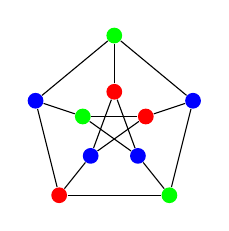
\begin{tikzpicture}[red/.style={circle,fill=red,inner sep=0pt,minimum size=2mm},blue/.style={circle,fill=blue,inner sep=0pt,minimum size=2mm},green/.style={circle,fill=green,inner sep=0pt,minimum size=2mm}]
	\node[red]												(1)	{};
	\node[green,node distance=1mm,below=of 1,xshift=-4mm]	(2)	{};
	\node[red,node distance=1mm,below=of 1,xshift=4mm]		(3)	{};
	\node[blue,node distance=6mm,below=of 1,xshift=-3mm]	(4)	{};
	\node[blue,node distance=6mm,below=of 1,xshift=3mm]		(5)	{};

	\node[green,node distance=5mm,above=of 1]				(11){};
	\node[blue,node distance=-1mm,below=of 1,xshift=-10mm]	(12){};
	\node[blue,node distance=-1mm,below=of 1,xshift=10mm]	(13){};
	\node[red,node distance=11mm,below=of 1,xshift=-7mm]	(14){};
	\node[green,node distance=11mm,below=of 1,xshift=7mm]	(15){};

	\draw (1) -- (4);
	\draw (1) -- (5);
	\draw (2) -- (3);
	\draw (2) -- (5);
	\draw (3) -- (4);

	\draw (1) -- (11);
	\draw (2) -- (12);
	\draw (3) -- (13);
	\draw (4) -- (14);
	\draw (5) -- (15);

	\draw (11) -- (12);
	\draw (11) -- (13);
	\draw (12) -- (14);
	\draw (13) -- (15);
	\draw (14) -- (15);
\end{tikzpicture}
\end{document}
